\chapter{Theoretical Framework}
\label{chapter:theoretical-framework}

\epigraph{``Another quote goes here''}{\vspace{10pt}Other author}

\newpage

This chapter describes the theoretical concepts needed to understand the work developed in the research effort and the related work that has been developed in the study field.


\section{Concept 1}

\label{section:Concept1}

First theoretical framework concept goes here.

\subsection{Subsection of Concept 1} 
\subsection{Subsection 2 of Concept 1}
Some text goes here \cite{examplereference}. An example of displaying and referencing an image is shown in \textbf{Figure \ref{fig:example}}


\begin{figure}
	\begin{center}
		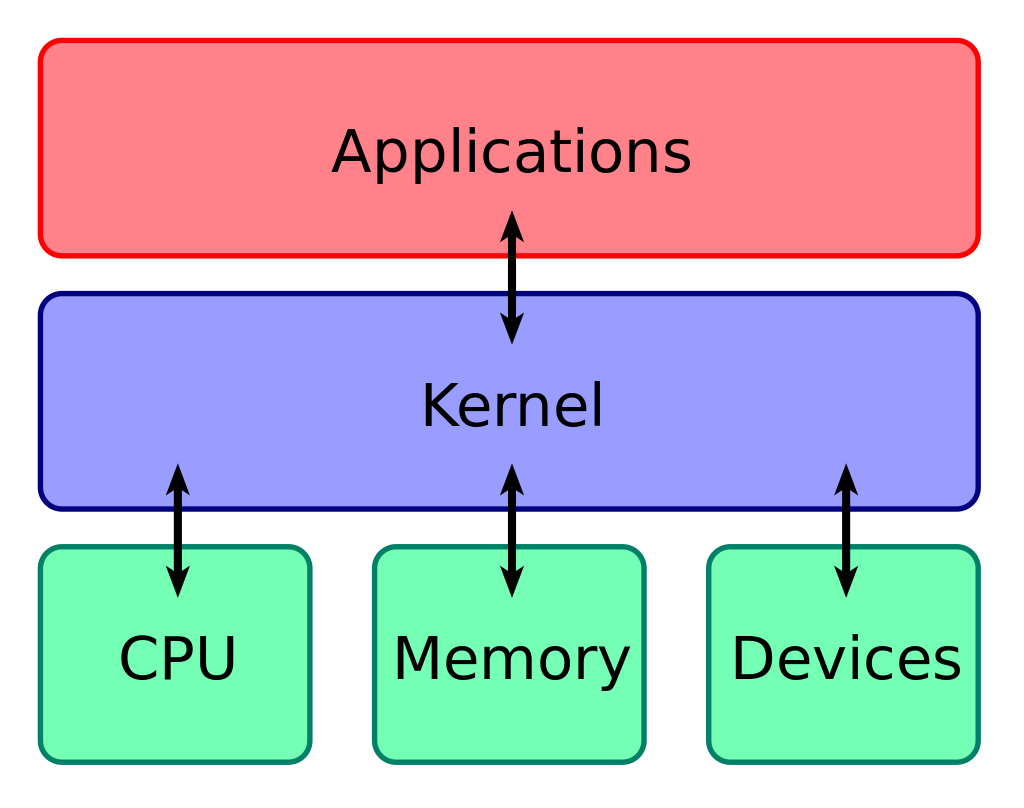
\includegraphics[width=1\columnwidth]{../img/image.png}
		\caption[]{Example image with reference \cite{examplereference}.}
		\label{fig:example}
	\end{center}
\end{figure}


\section{Concept 2}

\label{section:Concept2}

\subsection{Subsection Concept 2}

\subsubsection{Subsection 2 Concept 2}

\section{Concept 3}
An example of pseudo-code can be seen in \textbf{Algorithm \ref{examplepseudocode}}

\begin{pseudocode}{Pseudo\_Code}{Input} \label{examplepseudocode}
	\FOR y \GETS 1 \TO Input.MaxL \DO
	\BEGIN
	\FOR x \GETS 1 \TO Input.MaxH \DO
	\BEGIN
	a \GETS \CALL {FunctionCall}{x,y}\\
	b \GETS \CALL {AnotherFunction}{x, y}\\
	\CALL {ThirdFunction}{a,b}
	\END
	\END
\end{pseudocode}


\subsection{Example equation}
 Equation \ref{eq:1} shows an example equation.

\[
I=(L\cdot N) \tag{1} \label{eq:1}
\]
  
\section{Related Work}
%The related work for the research is include in this section \cite{examplereference}.

The related work for the research is included in this section:

Facial expression recognition (FER) has been extensively studied over the past decades, evolving from traditional machine learning approaches to deep learning methods. Early FER systems relied on handcrafted features such as Local Binary Patterns (LBP) and Histogram of Oriented Gradients (HOG). These approaches, while computationally efficient, often struggled to generalize across diverse datasets due to limited feature representation capabilities. 

The advent of convolutional neural networks (CNNs) revolutionized FER by enabling automatic feature extraction, with architectures such as VGGNet, ResNet \cite{he_deep_2015}, and EfficientNet achieving significant performance improvements. However, CNNs face limitations in capturing global dependencies and spatial relationships in images, which has motivated the exploration of transformer-based models in computer vision tasks \cite{islam_recent_2023}.

The introduction of Vision Transformers (ViTs) by Dosovitskiy \cite{dosovitskiy_image_2021} marked a significant shift in how visual tasks are approached. By leveraging self-attention mechanisms, ViTs can model long-range dependencies and capture richer contextual information compared to traditional CNNs.


In recent work on Facial Expression Recognition (FER), several models have demonstrated promising results, each with its unique strengths and limitations. ResNet-50 \cite{he_deep_2015} , a baseline convolutional neural network (CNN), performs well in local feature extraction, achieving an accuracy of 86.34\%. However, it struggles with capturing global context, which limits its effectiveness in more complex FER scenarios. The Swin Transformer \cite{liu_swin_2021}, with its hierarchical design, leverages both local and global features but comes with significant computational expense, resulting in an accuracy of 90.97\%. The Vision Transformer (ViT) Base \cite{dosovitskiy_image_2021} model, though powerful, has difficulty handling subtle FER cues in real-world conditions, also achieving an accuracy of 86.34\%. In contrast, the POSTER model \cite{zheng_poster_2022} achieves a superior accuracy of 92.05\% by combining pyramid attention with cross-fusion mechanisms, enabling the synergy of local and global features, which enhances its performance in FER tasks. 


\begin{table}[H]
\centering
\caption{State of the Art of FER systems}
\renewcommand{\arraystretch}{1.5} % Adjust row spacing
\begin{tabular}{llll}
\hline
\textbf{Model}   & \textbf{Accuracy (\%)} & \textbf{Parameters (M)} & \textbf{Key Insights}                                                                                                       \\ \hline
ResNet-50   \cite{he_deep_2015}     & 86.34                  & 24.6 & \begin{tabular}[c]{@{}l@{}}Baseline CNN with strong local \\ feature extraction but lacks \\ global context.\end{tabular}   \\
Swin Transformer \cite{liu_swin_2021} & 90.97                & 28.3                    & \begin{tabular}[c]{@{}l@{}}Hierarchical ViT with local-global \\ features but computationally \\ expensive.\end{tabular}    \\
ViT (Base)  \cite{dosovitskiy_image_2021}     & 86.34                 & 86.4               & \begin{tabular}[c]{@{}l@{}}Transformer struggles \\ with subtle FER cues in \\ real-world conditions.\end{tabular} \\
\textbf{POSTER} \cite{zheng_poster_2022}  & \textbf{92.05}         & \textbf{Not specified}           & \begin{tabular}[c]{@{}l@{}}Combines pyramid attention and \\ cross-fusion for local-global \\ feature synergy.\end{tabular} \\ \hline
\end{tabular}
\end{table}


